\documentclass[11pt]{article}
\usepackage{fontspec}
\setmainfont{DejaVu Serif}
\usepackage[margin=1cm,landscape]{geometry}
\usepackage{longtable}
\usepackage{array}
\usepackage{graphicx}
\usepackage{xcolor}
\pagestyle{plain}

\newcolumntype{L}[1]{>{\raggedright\arraybackslash}p{#1}}

\setlength{\tabcolsep}{6pt}
\renewcommand{\arraystretch}{1.15}
\setlength{\parindent}{0pt}
\setlength{\parskip}{5pt}
\setlength{\fboxsep}{2pt}
\setlength{\fboxrule}{0.6pt}
\definecolor{slideframe}{gray}{0.55}
\renewcommand{\fbox}[1]{{\fcolorbox{slideframe}{white}{#1}}}

\begin{document}

{\LARGE\bfseries Текст выступления --- «Спокуха»}
\vspace{0.5em}

\begin{longtable}{L{2.6cm} L{8cm} L{14.7cm}}
\textbf{Слайд} & \textbf{Скриншот} & \textbf{Текст} \\
\hline
\endhead

\textbf{1}\newline \textit{\small\textasciitilde 20 сек} &
\fbox{
\includegraphics[width=7.5cm]{slides/slide-01.png}} &
Здравствуйте, уважаемые члены экспертной комиссии! Мы — команда «Спокойствие, только спокойствие».

«Спокуха» возвращает дежурным спокойствие: среди тысяч событий она показывает нужному человеку именно то, на что действительно нужно реагировать.
\\
\hline

\textbf{2}\newline \textit{\small\textasciitilde 25 сек} &
\fbox{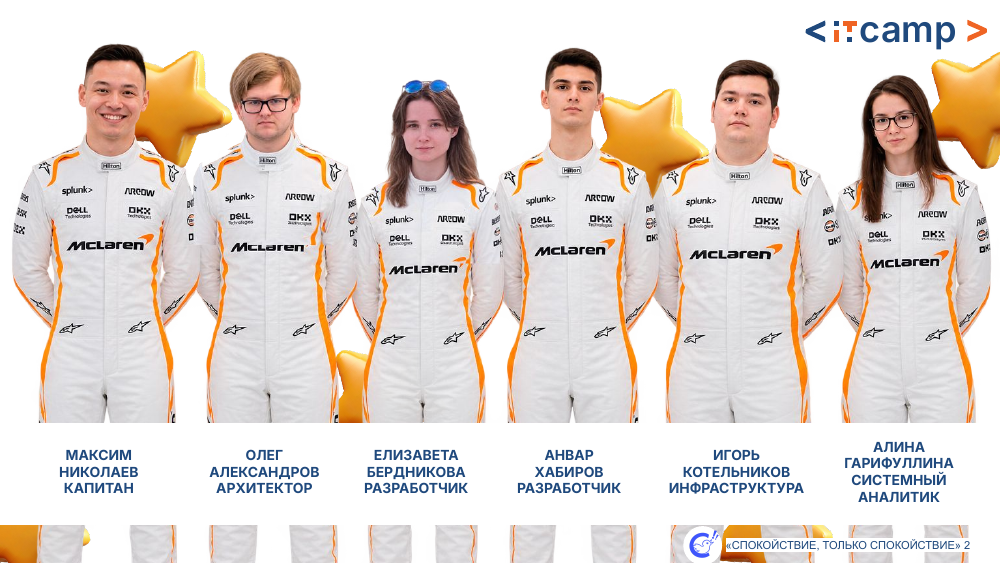
\includegraphics[width=7.5cm]{slides/slide-02.png}} &
Перед вами команда, работавшая над решением. Нас шесть человек, и мы закрываем полный цикл: от бизнес-анализа и архитектуры до разработки, инфраструктуры и безопасности. Такой состав позволил посмотреть на задачу сразу с нескольких сторон — не только с технической, но и со стороны пользователя и реальной эксплуатации.
\\
\hline

\textbf{3}\newline \textit{\small\textasciitilde 35 сек} &
\fbox{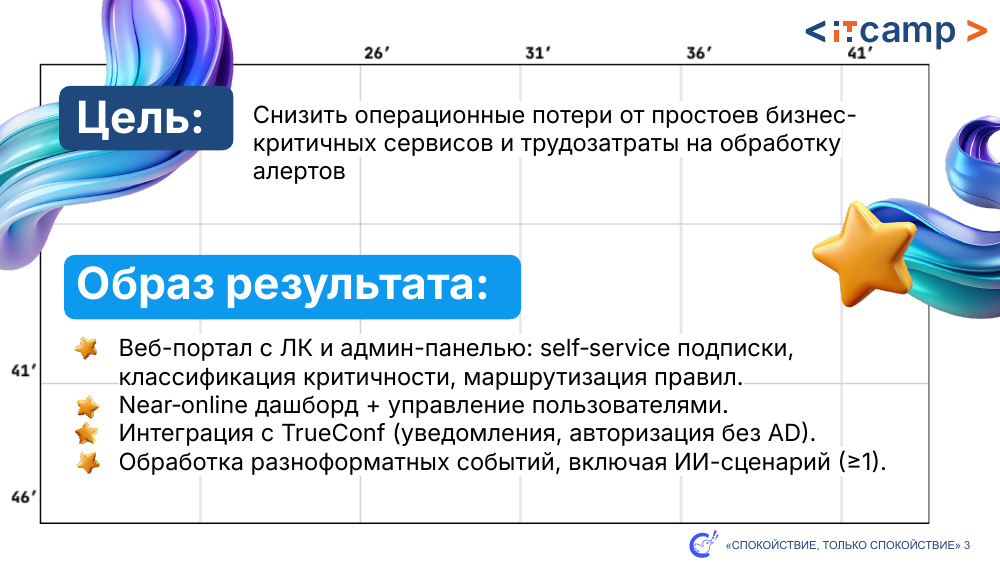
\includegraphics[width=7.5cm]{slides/slide-03.png}} &
На слайде — стоящая перед проектом бизнес-цель: снизить потери от простоев бизнес-критичных сервисов и сократить ручную обработку алертов.

Вытекающий из неё образ результата — единая платформа. Это веб-портал с личным кабинетом и панелью администратора, где сотрудник сам настраивает себе подписки, а администратор — классификацию критичности и правила маршрутизации; сводная панель, обновляющаяся почти в реальном времени, с управлением пользователями; интеграция с TrueConf сразу для двух задач — доставки уведомлений и входа в систему без корпоративного каталога; и обработка разноформатных событий как минимум с одним рабочим ИИ-сценарием. Инженер получает не поток сырых алертов, а уже отфильтрованную картину происходящего.
\\
\hline

\textbf{4}\newline \textit{\small\textasciitilde 40 сек} &
\fbox{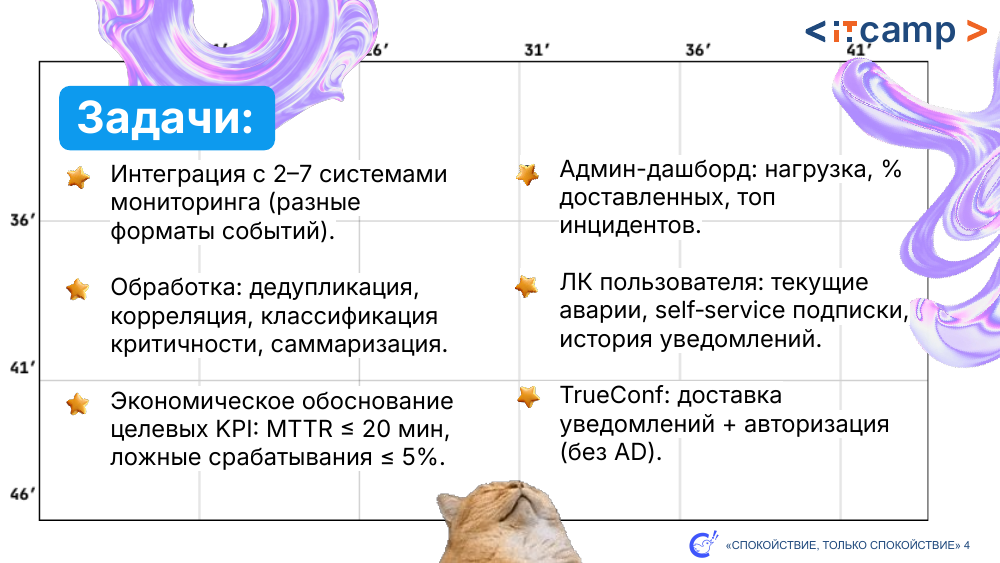
\includegraphics[width=7.5cm]{slides/slide-04.png}} &
Вынесенные на слайд задачи делятся на две части. Слева — то, что система принимает и обрабатывает. Это интеграция с двумя-семью системами мониторинга, и у каждой свой формат событий. Дальше обработка: дедупликация, корреляция, классификация критичности и саммаризация. И экономическое обоснование целевых показателей: время реакции не больше двадцати минут, ложные срабатывания не выше пяти процентов.

Справа — то, что видит человек. Панель администратора показывает нагрузку, долю доставленных уведомлений и самые частые инциденты. Личный кабинет показывает текущие аварии и историю уведомлений, там же сотрудник сам настраивает подписки. А TrueConf закрывает сразу две задачи: доставку и вход в систему без корпоративного каталога.
\\
\hline

\textbf{5}\newline \textit{\small\textasciitilde 55 сек} &
\fbox{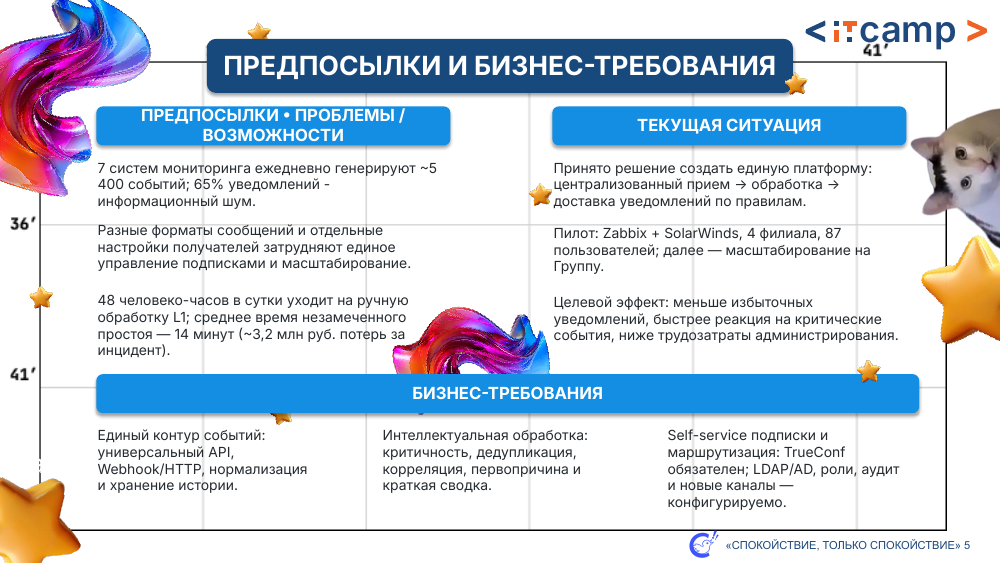
\includegraphics[width=7.5cm]{slides/slide-05.png}} &
Приведённые на слайде цифры обнажают масштаб проблемы: семь систем мониторинга генерируют около 5400 событий в сутки, 65\% из них — шум, а разные форматы сообщений и разрозненные настройки получателей затрудняют единое управление подписками.

Уходящие на разбор 48 человеко-часов в сутки — ещё не главная беда. Хуже другое: простой остаётся незамеченным в среднем 14 минут, и это стоит около 3,2 миллиона рублей за инцидент.

Отсюда и принятое решение: единая платформа с централизованным приёмом, обработкой и доставкой по правилам. Разворачиваемый уже сейчас пилот охватывает четыре филиала и около 87 пользователей — это не лабораторный стенд, а боевой контур с реальными данными, дальше — масштабирование на всю группу компаний.
\\
\hline

\textbf{6}\newline \textit{\small\textasciitilde 50 сек} &
\fbox{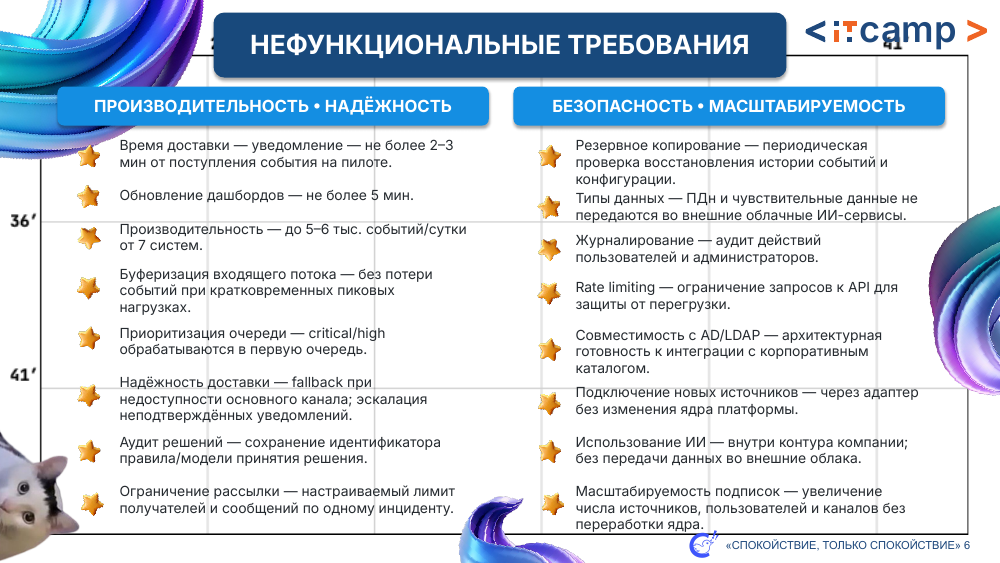
\includegraphics[width=7.5cm]{slides/slide-06.png}} &
Собранные здесь требования к платформе делятся на два блока. Слева — производительность и надёжность. Уведомление доставляется за 2--3 минуты, сводная панель обновляется не дольше 5 минут. Платформа держит до пяти-шести тысяч событий в сутки от семи систем и копит входящий поток в буфере, чтобы не терять события на пиках. Критичные алерты обрабатываются в первую очередь. Если основной канал недоступен, работает резервный, а неподтверждённые уведомления эскалируются. И по каждому решению сохраняется, какое именно правило или модель его приняли.

Справа — безопасность и масштабируемость. Персональные и чувствительные данные не уходят во внешние ИИ-сервисы, сам ИИ работает внутри контура компании. Действия пользователей и администраторов журналируются. Ограничение частоты запросов защищает платформу от перегрузки. Резервное копирование дополнено периодической проверкой восстановления. Архитектура готова к подключению корпоративного каталога Active Directory, а новые источники подключаются адаптером без изменения ядра. Значит, при росте компании платформа растёт вместе с ней, а не требует пересборки с нуля.
\\
\hline

\textbf{7}\newline \textit{\small\textasciitilde 25 сек} &
\fbox{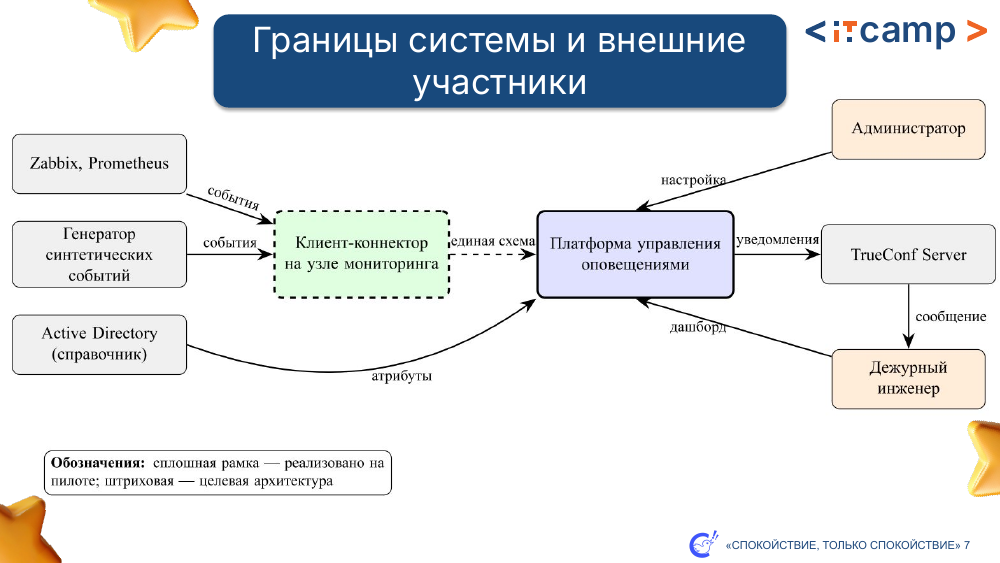
\includegraphics[width=7.5cm]{slides/slide-07.png}} &
Показанная на схеме архитектура помещает платформу между источниками и получателем. Слева входят события — Zabbix, Prometheus и генератор синтетических событий — через коннектор на узле мониторинга.

Платформа определяет получателя и уведомляет дежурного инженера через TrueConf. Справа картину дополняют ещё два участника: администратор, который настраивает правила, и Active Directory, который хранит данные о пользователях. Сплошная рамка на схеме — уже реализованное на пилоте, штриховая — целевая архитектура.
\\
\hline

\textbf{8}\newline \textit{\small\textasciitilde 20 сек} &
\fbox{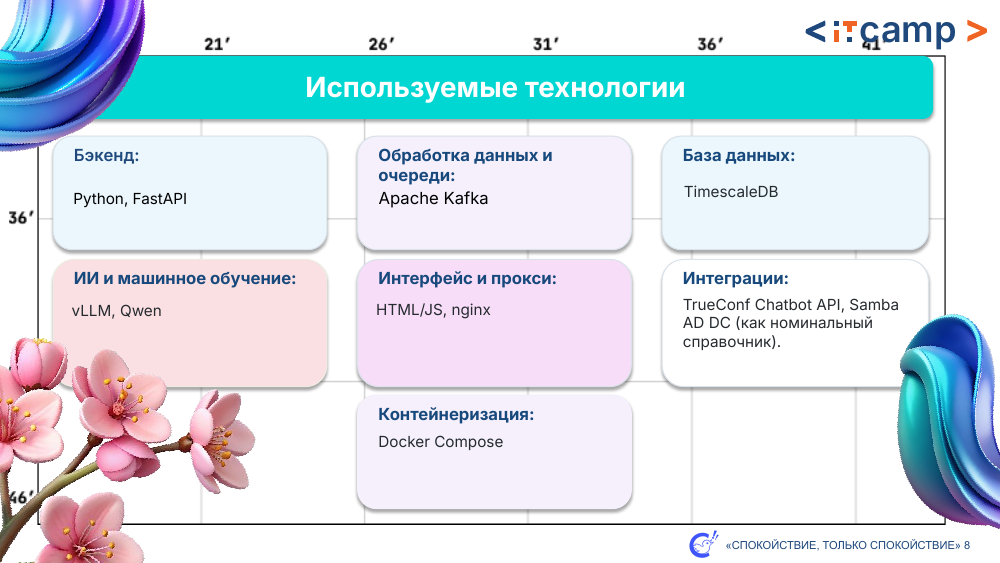
\includegraphics[width=7.5cm]{slides/slide-08.png}} &
Представленный на слайде стек выбирался как достаточно простой и промышленно применимый: Python и FastAPI в серверной части, Kafka для обмена событиями, TimescaleDB для хранения, локальный ИИ на vLLM и Qwen, интерфейс на nginx. Все компоненты упакованы в Docker-контейнеры.
\\
\hline

\textbf{9}\newline \textit{\small\textasciitilde 50 сек} &
\fbox{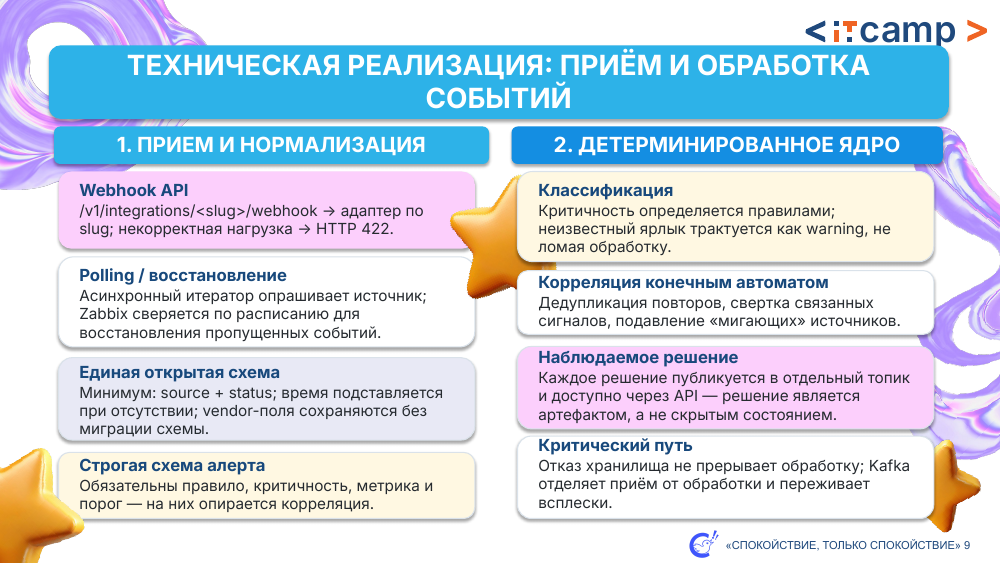
\includegraphics[width=7.5cm]{slides/slide-09.png}} &
Попадающее в систему событие сначала проходит приём. Слева на слайде четыре его составляющие. Первая — точка приёма: источник присылает событие сам, нужный адаптер определяется по имени источника прямо в адресе, а некорректные данные отклоняются кодом 422. Вторая — периодический опрос, например сверка с Zabbix по расписанию, чтобы восстановить пропущенные события. Третья — единая открытая схема: обязательны только источник и статус, а поля вендора сохраняются как есть, без миграции схемы. Четвёртая — строгая схема алерта: правило, критичность, метрика и порог обязательны, потому что на них опирается корреляция.

Дальше работает детерминированное ядро. Критические решения принимает система правил, а не нейросеть. Она классифицирует критичность по заданным порогам, причём неизвестная метка трактуется как предупреждение и не ломает обработку. Она убирает дубли, объединяет связанные сигналы конечным автоматом и подавляет «мигающие» источники. Каждое решение публикуется отдельно и доступно для проверки. Значит, при сбое команда быстро находит причину и точечно донастраивает правило, а не гадает вслепую. Отказ хранилища обработку не прерывает: Kafka отделяет приём от обработки и переживает всплески.
\\
\hline

\textbf{10}\newline \textit{\small\textasciitilde 55 сек} &
\fbox{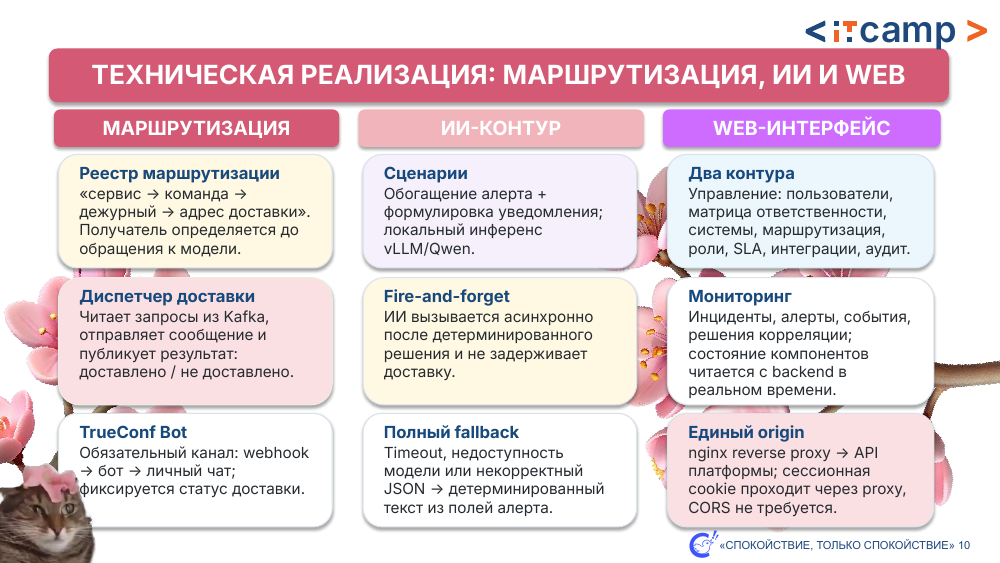
\includegraphics[width=7.5cm]{slides/slide-10.png}} &
Определяемый ещё до обращения к модели маршрут выглядит так: сервис, ответственная команда, дежурный, адрес доставки. Диспетчер доставки читает запросы из Kafka, отправляет сообщение и публикует результат: доставлено или не доставлено. Обязательным каналом остаётся бот TrueConf. Он принимает запрос и пишет в личный чат, а статус доставки фиксируется.

Подключаемый только затем ИИ работает асинхронно, по принципу «отправил и забыл». Он обогащает алерт и формулирует понятное уведомление, но не задерживает доставку ни на секунду.

Отказ модели нам не страшен. Она может стать недоступной, зависнуть или ответить ошибкой — уведомление всё равно уйдёт. Просто текст соберёт резервный путь, детерминированным способом из полей самого алерта.

Справа на слайде веб-интерфейс, и он делится на два контура. Контур управления — это пользователи, матрица ответственности, системы, роли, маршрутизация, сроки реакции, интеграции и аудит. Контур мониторинга — инциденты, алерты, события и решения корреляции. Состояние компонентов читается с серверной части в реальном времени. Работает всё это через единый адрес: браузер обращается только к nginx, а тот уже передаёт запрос платформе. Поэтому сессионный ключ проходит насквозь и дополнительных настроек не требуется.
\\
\hline

\textbf{11}\newline \textit{\small\textasciitilde 45 сек} &
\fbox{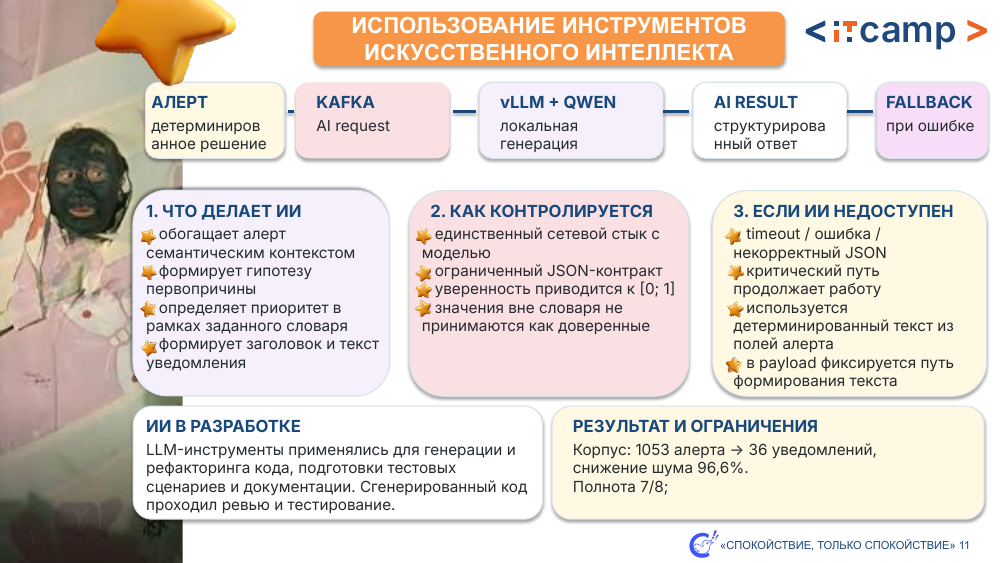
\includegraphics[width=7.5cm]{slides/slide-11.png}} &
Выполняющий четыре задачи ИИ добавляет семантический контекст, гипотезу первопричины, приоритет в рамках заданного словаря и понятный человеку заголовок с текстом уведомления. При этом формат ответа задан строго, а менять логику системы модель не имеет права: значения вне словаря просто не принимаются как доверенные.

ИИ помогал и в самой разработке: он генерировал и рефакторил код. Но весь такой код проходил ревью и тестирование.

Достигнутый на прототипе результат впечатляет: на тестовом корпусе из 1053 алертов система формирует всего 44 уведомления, то есть шум сократился на 95,8\%. На слайде стоит цифра 36 — это более ранняя версия. Там же честно указана её полнота: семь инцидентов из восьми. Один инцидент терялся, и мы это исправили. Система стала отправлять на восемь сообщений больше, зато теперь находит все восемь инцидентов из восьми: для системы оповещения полнота важнее красивого процента.
\\
\hline

\textbf{12}\newline \textit{\small\textasciitilde 45 сек} &
\fbox{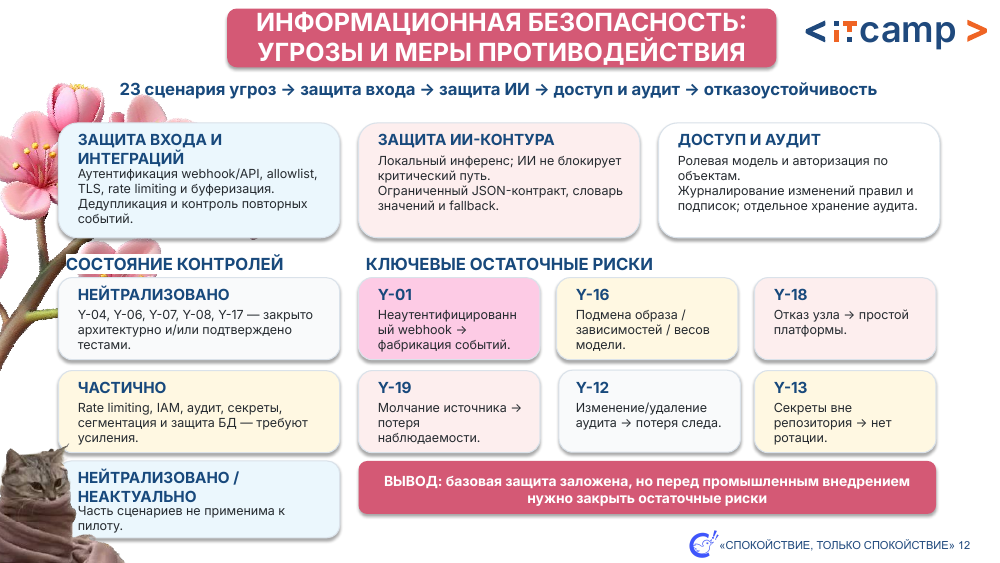
\includegraphics[width=7.5cm]{slides/slide-12.png}} &
Разобранные 23 сценария угроз сгруппированы по зонам защиты. Вход и интеграции — проверка подлинности источника, список разрешённых адресов, шифрование канала, ограничение частоты запросов, буферизация и контроль повторных событий. Контур самого ИИ: модель работает внутри контура компании, ответ принимается в строго заданном формате и только в пределах словаря допустимых значений, а на любой сбой предусмотрен резервный путь. Доступ и аудит: ролевая модель с авторизацией по объектам, журналирование изменений правил и подписок, отдельное хранение аудита.

Шесть угроз закрыты архитектурно и подтверждены тестами — это как раз весь ИИ-контур. Ключевые остаточные риски мы называем прямо, они перечислены на слайде. Точка приёма событий пока не проверяет подлинность источника, то есть событие можно подделать. Возможна подмена образа, зависимостей или весов модели. Узел у нас один, и его отказ останавливает платформу. Молчание источника мы пока не отслеживаем, а значит можем потерять наблюдаемость. Записи аудита можно изменить или удалить. И секреты лежат вне репозитория, но не ротируются. Заложенная базовая защита — это фундамент, но перед промышленным внедрением эти риски нужно закрыть.
\\
\hline

\textbf{13}\newline \textit{\small\textasciitilde 25 сек} &
\fbox{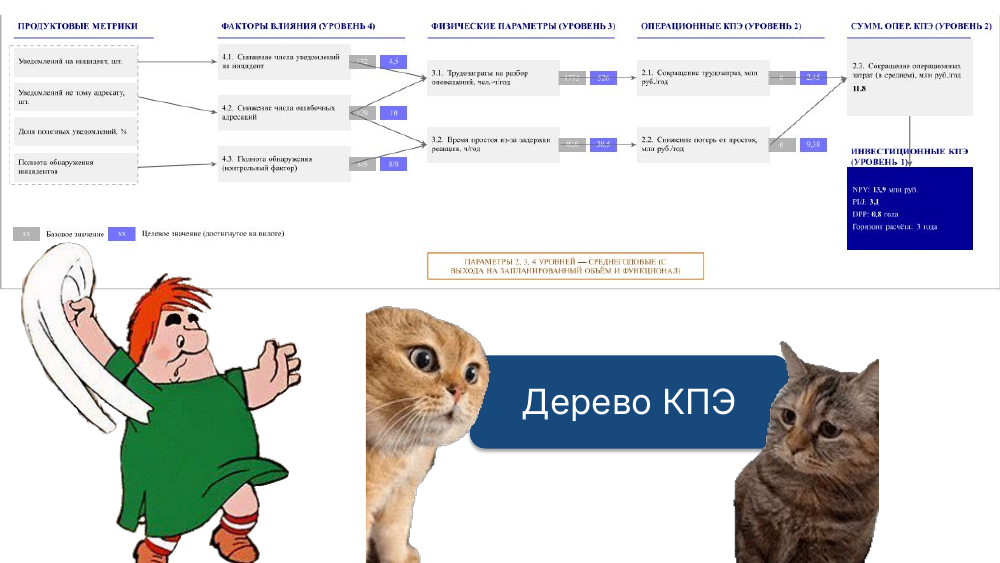
\includegraphics[width=7.5cm]{slides/slide-13.png}} &
Показанное на слайде дерево КПЭ связывает продуктовые метрики с операционными и финансовыми и показывает всю цепочку в цифрах. Число уведомлений на инцидент падает со 132 до пяти с половиной. Это экономит около 2,45 миллиона рублей трудозатрат в год и ещё 9,38 миллиона на сокращении потерь от простоя, вместе — около 11,8 миллиона рублей операционной экономии ежегодно. Рассчитанные на этой основе инвестиционные показатели подтверждают: технология здесь работает не сама на себя, а на бизнес-результат. Чистая приведённая стоимость — 13,9 миллиона рублей, окупаемость — 0,8 года.
\\
\hline

\textbf{14}\newline \textit{\small\textasciitilde 28 сек} &
\fbox{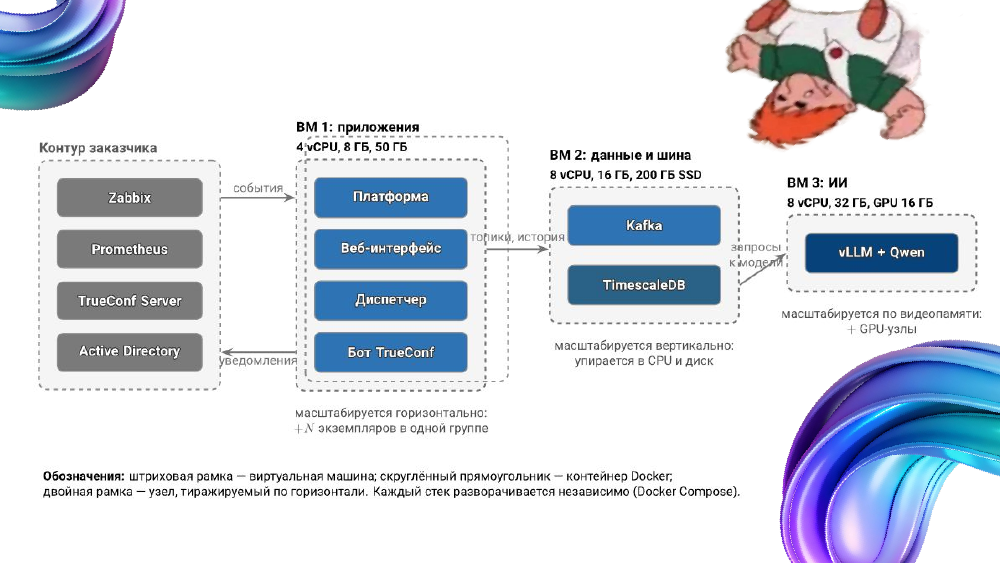
\includegraphics[width=7.5cm]{slides/slide-14.png}} &
Спроектированная для пилота инфраструктура делится на три виртуальные машины, и каждая масштабируется независимо: приложения, данные вместе с шиной событий и отдельно ИИ с видеокартой. Вокруг них — контур заказчика с источниками событий.

Каждый блок растёт по-своему. Приложения растут горизонтально, добавлением экземпляров. Данные растут вертикально. ИИ упирается в видеопамять, поэтому растёт добавлением узлов с видеокартами. Подключение новых систем или подразделений не требует останавливать платформу, а вложения не устаревают по мере роста бизнеса.
\\
\hline

\textbf{15}\newline \textit{\small\textasciitilde 30 сек} &
\fbox{
\includegraphics[width=7.5cm]{slides/slide-15.png}} &
Итак, «Спокуха» превращает поток из тысяч событий в горстку понятных, адресных уведомлений — быстрее реакция, меньше шума, и ИИ не становится точкой отказа.

Отдельно — три вещи, которыми мы гордимся: она измерима, поэтому её быстро и дёшево донастраивают; она обкатана на реальном боевом контуре, а не в воображении; и она растёт вместе с бизнесом, без переработки ядра.

Как говорил Карлсон: «Спокойствие, только спокойствие». Спасибо!
\\
\hline
\end{longtable}

\end{document}
